\documentclass[12pt, a4paper]{article}
\usepackage{titling}
\usepackage[hidelinks=true]{hyperref}
\usepackage{graphicx}
\usepackage{appendix}
\usepackage{tabularx}


\newcolumntype{b}{X}
\newcolumntype{s}{>{\hsize=.5\hsize}X}
\newcommand{\heading}[1]{\multicolumn{1}{c}{#1}}

\newcommand{\email}[1]{
  \small{\textit{\href{mailto:#1}{#1}}}
}

\title{
  \huge\textbf{MXEN 2002} \\
  \vspace{2em}
  \large\textbf{Project Report}\\
  \vspace{0.5em}
}

\preauthor{
  \vspace{12cm}
  \begin{center}
    \begin{tabular}[t]{c}
}

\author{
    \textbf{Kee-An Seet} \\
    \email{19776219@student.curtin.edu.au} \\
    \textbf{Harry Cassidy} \\
    \email{20607591@student.curtin.edu.au}
}

\postauthor{
    \end{tabular}
    \par
  \end{center}
}

\date{}

\begin{document}
\pagenumbering{gobble}
\maketitle
\pagebreak

\pagenumbering{roman}
\tableofcontents
\paragraph{}
\newpage
\listoffigures
\paragraph{}
\listoftables
\paragraph{}
\pagebreak

\pagenumbering{arabic}

\section{Nomenclature}\label{sec:nomen}
\paragraph{}

\newpage
\section{The Task} \label{sec:intro}

\paragraph{}
  We were tasked with building, wiring, and programming a robot to complete a series of objectives, such as navigating a maze autonomously and moving a camera with a servo as to let the operator identify targets. We were to use the Arduino Mega hardware with a DC motor drive system along with several distance sensors to help achieve the objectives.

\begin{figure}[h]
  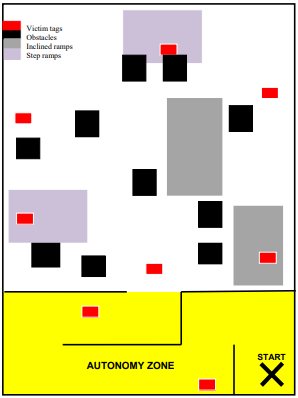
\includegraphics{Images/AutonZone.png}
  \centering
  \caption{Supplied example of the task map}
  \label{fig:intro:map}
\end{figure}

\subsection{Autonomy Zone}
  \paragraph{}
    The "Autonomy Zone" is the section of the map in which the robot is completely self controlled. The idea behind this challenge is that in the event of a connection dsiruption in a dangerous area for humans, the robot should be able to rescue it's self from danger.

\subsection{Manual Control}
 \paragraph{}
    The majority of the task is to control the robot through wireless communication. During this period the robot (controlled by the user) must drive through the zone and send a camera feed back to the user for "victim" tags to be recorded.


\newpage

\section{Our Solution} \label{sec:Solution}
  \subsection{Overview}
    \paragraph{}
      Mechanically constructed from the supplied robot base. It has two driving motors each attached 
      to tank treads, on top there is a platform with mounting holes for an Arduino Mega and various 
      sensor brackets. Initially our plan was to use the given prototyping breadboard with limited modification 
      to the drivebase, however after some testing we identified several issues with this. The final product we 
      created used a more permanent Arduino "Shield" that we created with a solder on prototyping board.

  \subsection{Issues and Solutions}
    \paragraph{}
      Before starting we identified several potential issues and solutions that we thought may impact 
      our project, listed below:

    \begin{table}[htbp]
       \centering
        \begin{tabularx}{\textwidth}{bb}
            \hline
            \heading{Issue} & \heading{Solution} \\ \hline
            During Lab G we found that the tracks would fall off if run too long as the nut would unscrew and as such unbolt the wheel & Initially we intended on using locktite, however we didn't want to use a potentiallly damaging product, to solve this issue we opted to use a second nut on each bolt to reduce the effect of vibration \\ \hline
            We found throughout our labs we found that we had many issues with the wiring and using the breadboards as the connections were loose & To remedy this we planned out our circuit and soldered a "prototyping shield" for an Arduino Mega to create our own "MXEN2002 shield" \\ \hline
            The front sensor didnt have the resolution to sense the in front of the robot from its initial position & We moved the sensor mounting around as to position it below the robot and sunk back slightly \\ \hline
        \end{tabularx}
      \caption{Issues + Solutions}
    \end{table}

\end{document}